\documentclass[10pt,a4paper]{article}
\usepackage[T1]{fontenc}
\usepackage{lmodern,graphicx,booktabs,tabularx,array,xcolor,hyperref,geometry}
\geometry{left=21mm,right=21mm,top=18mm,bottom=20mm}
\definecolor{ink}{HTML}{172B40}
\definecolor{blue}{HTML}{17636E}
\hypersetup{colorlinks=true,urlcolor=blue,linkcolor=blue,pdftitle={A candidate depression northwest of McGetchin crater}}
\setlength{\parindent}{0pt}
\setlength{\parskip}{5pt}
\newcommand{\tagline}[1]{{\sffamily\color{blue}\small\bfseries #1}\par}
\newcommand{\heading}[1]{{\sffamily\color{ink}\Large\bfseries #1}\par}
\newcommand{\subhead}[1]{\vspace{2pt}{\sffamily\color{ink}\bfseries #1}\par}
\newcommand{\figcap}[1]{{\footnotesize\color{ink}#1}\par}
\begin{document}
\tagline{LUNAR RECONNAISSANCE ORBITER \hfill 20 NOVEMBER 2026}
{\sffamily\color{ink}\fontsize{24}{28}\selectfont\bfseries A candidate depression northwest\\of McGetchin crater\par}
\vspace{3pt}
A compact hollow about 5 m across appears at \textbf{1.36151$^\circ$ N, 67.16426$^\circ$ E}, 442 m northwest of the center of the 222 m McGetchin crater. Stereo images and repeated observations with opposite sunlight support newly expressed relief. Raised material beside the hollow is consistent with a gap or slope between newly deposited clumps of ejecta. Neither a continuous rim nor excavation by a separate projectile is established.

\begin{center}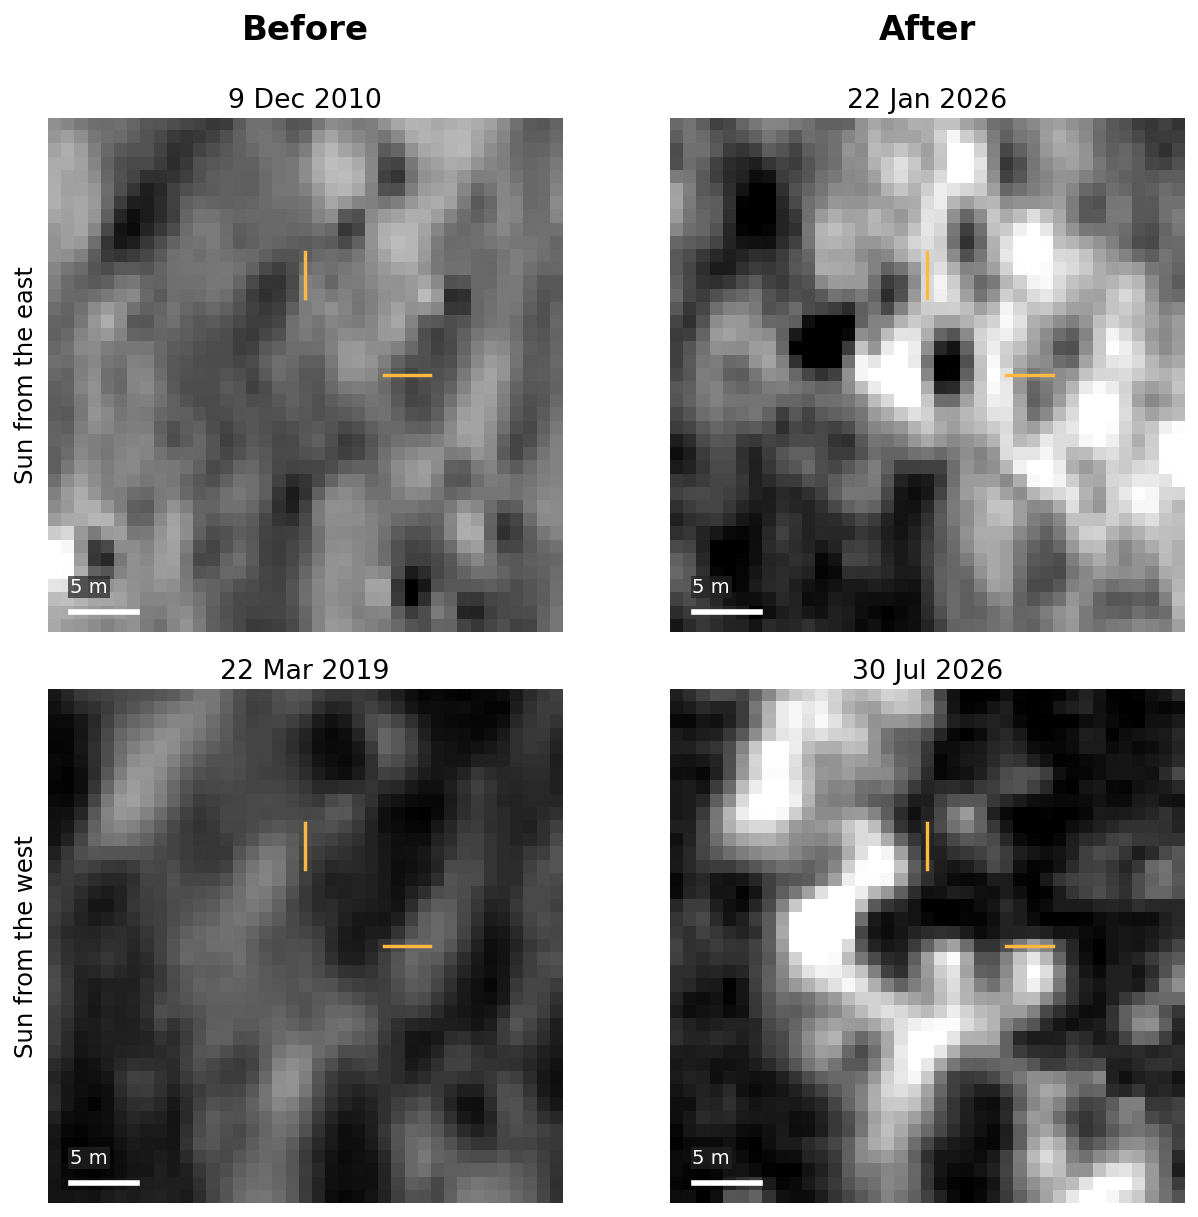
\includegraphics[width=.73\linewidth]{mcgetchin-walls.png}\end{center}
\figcap{\textbf{Figure 1.} Each panel shows the same 39 m square, north up. The amber ticks point to its center. Each row uses the same grayscale for both epochs after normalization to nearby terrain. Eastern-Sun incidences are 71$^\circ$ and 69$^\circ$. Western-Sun incidences are 80.47$^\circ$ and 82.69$^\circ$, with native pixels 0.83 and 0.95 m wide. The bright material to the west of the target is part of the ambiguity in interpreting the center. Images from NASA/GSFC and the LROC team.}

\subhead{What the dates establish}
The last diagnostic western-Sun image before the change is 22 March 2019. The center also appeared ordinary under high Sun on 9 April 2022. It was brighter by 28 November 2025, and three views on 25 December 2025 support a hollow. The separately published formation interval for the McGetchin primary is 11 April--22 May 2024. Dating this smaller feature to that same interval requires assuming an association. \href{https://doi.org/10.1126/sciadv.aeh7812}{Robinson et al.\ (2026)}.

\newpage
\tagline{MCGETCHIN \hfill LOCAL TOPOGRAPHY}
\heading{A local low beside raised material}
The comparable low-Sun pairs put the same wall under opposite lighting. A seven-scale search produced 85 spatially separated candidates. Six survived an opposite-Sun score threshold of 3, including this site. In two 3 m square apertures with centers separated by 4 m, the log brightness ratio of the western to eastern aperture changes from $-0.053$ to $+0.707$ under eastern Sun and from $+0.451$ to $-0.995$ under western Sun. A nearby old pit already displays the expected wall contrast in the before images. Seventy-two off-target terrain patches used in each low-Sun comparison have median registration offsets of zero on the 1 m grid.

\subhead{Sensitivity of the stereo measurement}
Three images from 25 December 2025 give three pairings that share the original views. After removing a local trend, the table gives the center height minus the median height of an annulus 4.4--7.2 m from the center. Negative values indicate a local low. These are image-matching estimates rather than absolute depth measurements.
\begin{center}
\begin{tabular}{lrrr}
\toprule
Matching window & East--west & East--nadir & Nadir--west \\
\midrule
5 pixels  & $-0.66$ m & $-0.73$ m & $-0.68$ m\\
7 pixels  & $-0.37$ m & $-0.51$ m & $-0.44$ m\\
9 pixels  & $-0.27$ m & $-0.47$ m & $-0.32$ m\\
11 pixels & $-0.12$ m & $-0.28$ m & $+0.07$ m\\
15 pixels & $+0.13$ m & $+0.11$ m & $+0.20$ m\\
\bottomrule
\end{tabular}
\end{center}
The larger windows mix the feature with its surroundings and reverse the sign. The published 3 m digital terrain model alone does not resolve the depression. Restoring this terrain model and fitting background planes 12--18 m away gives a central offset of $-0.24$ to $-0.49$ m, with the western flank raised by 0.57--0.78 m. The eastern flank ranges from $-0.42$ to $+0.10$ m. This asymmetry and the absence of a comparable pre-event elevation model at this resolution leave excavation uncertain. A ray traced toward the low western Sun also finds that raised material could shadow the western half. The eastern dark half has no corresponding resolved blocker in the sampled eastern terrain.

\subhead{Comparison with published features}
On a nominal overlay of Robinson et al.'s Figure 7, the position is about 7 m from a detached contour. The overlay has no independent boundary-error estimate. No individual crater or boulder symbol is centered there. The figure documents selected features. It cannot establish that nobody has seen the site. Among the 21 coordinate-bearing recent large craters tabulated by Powell et al., the nearest is McGetchin itself, at 442 m. The nearest entry in the 222-crater LROC change catalog is 217 km away. The latter catalog predates McGetchin. Neither list is a complete inventory of meter-scale secondary craters.

\begin{center}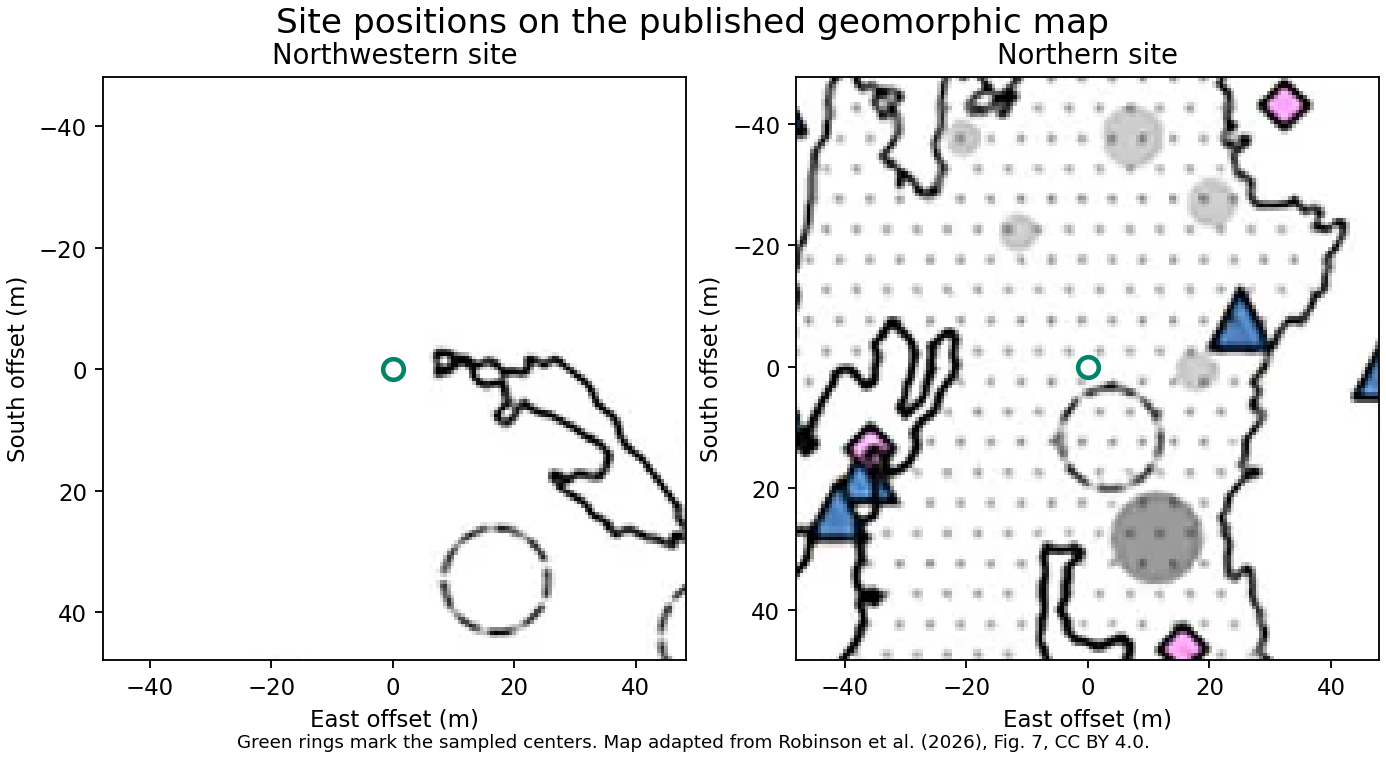
\includegraphics[width=.55\linewidth]{mcgetchin/published-map.png}\end{center}
\figcap{Green rings mark the sampled sites. The northwestern candidate is on the left. The northern comparison on the right is adjacent to an already mapped crater. Map adapted from Robinson et al., Figure 7, CC BY 4.0.}
\subhead{Finding the site in the source images}
In calibrated PDS image \href{https://data.lroc.im-ldi.com/lroc/view_lroc/LRO-L-LROC-3-CDR-V1.0/M1307882452LC}{M1307882452LC} (March 2019), its zero-based sample and line are 1108.81 and 23242.94. In \href{https://data.lroc.im-ldi.com/lroc/view_lroc/LRO-L-LROC-3-CDR-V1.0/M1540060927RC}{M1540060927RC} (July 2026) they are 377.90 and 25506.14. These image addresses identify the few relevant pixels more reliably than the final decimal places of a map coordinate.

\figcap{\href{https://zenodo.org/records/21481275}{Calibrated map products and terrain models} \quad
\href{https://data.lroc.im-ldi.com/lroc/view_rdr/SHAPEFILE_GLOBAL_NEW_CRATERS}{LROC temporal-crater catalog} \quad
\href{https://zenodo.org/records/19472800}{Powell et al.\ catalog} \quad
\href{https://zenodo.org/records/15755155}{Soko\l owska et al.\ data}}

\newpage
\tagline{ADDITIONAL FIELDS \hfill TIME AND ILLUMINATION CONTROLS}
\heading{A bright marking that predates the nearby flash}
At approximately \textbf{6.10273$^\circ$ S, 276.99227$^\circ$ E}, an independent marking appeared between 10 November 2022 (18:53:52 UTC) and 13 March 2023 (01:00:42 UTC). It was already present 73 calendar days before the NELIOTA flash of 25 May 2023, whose reported position is only 6.95 km away. The close spatial match would have produced a false association without the March and April images. \href{https://neliota.astro.noa.gr/LIFDatabase/EventDetails/363}{NELIOTA event record}.

\begin{center}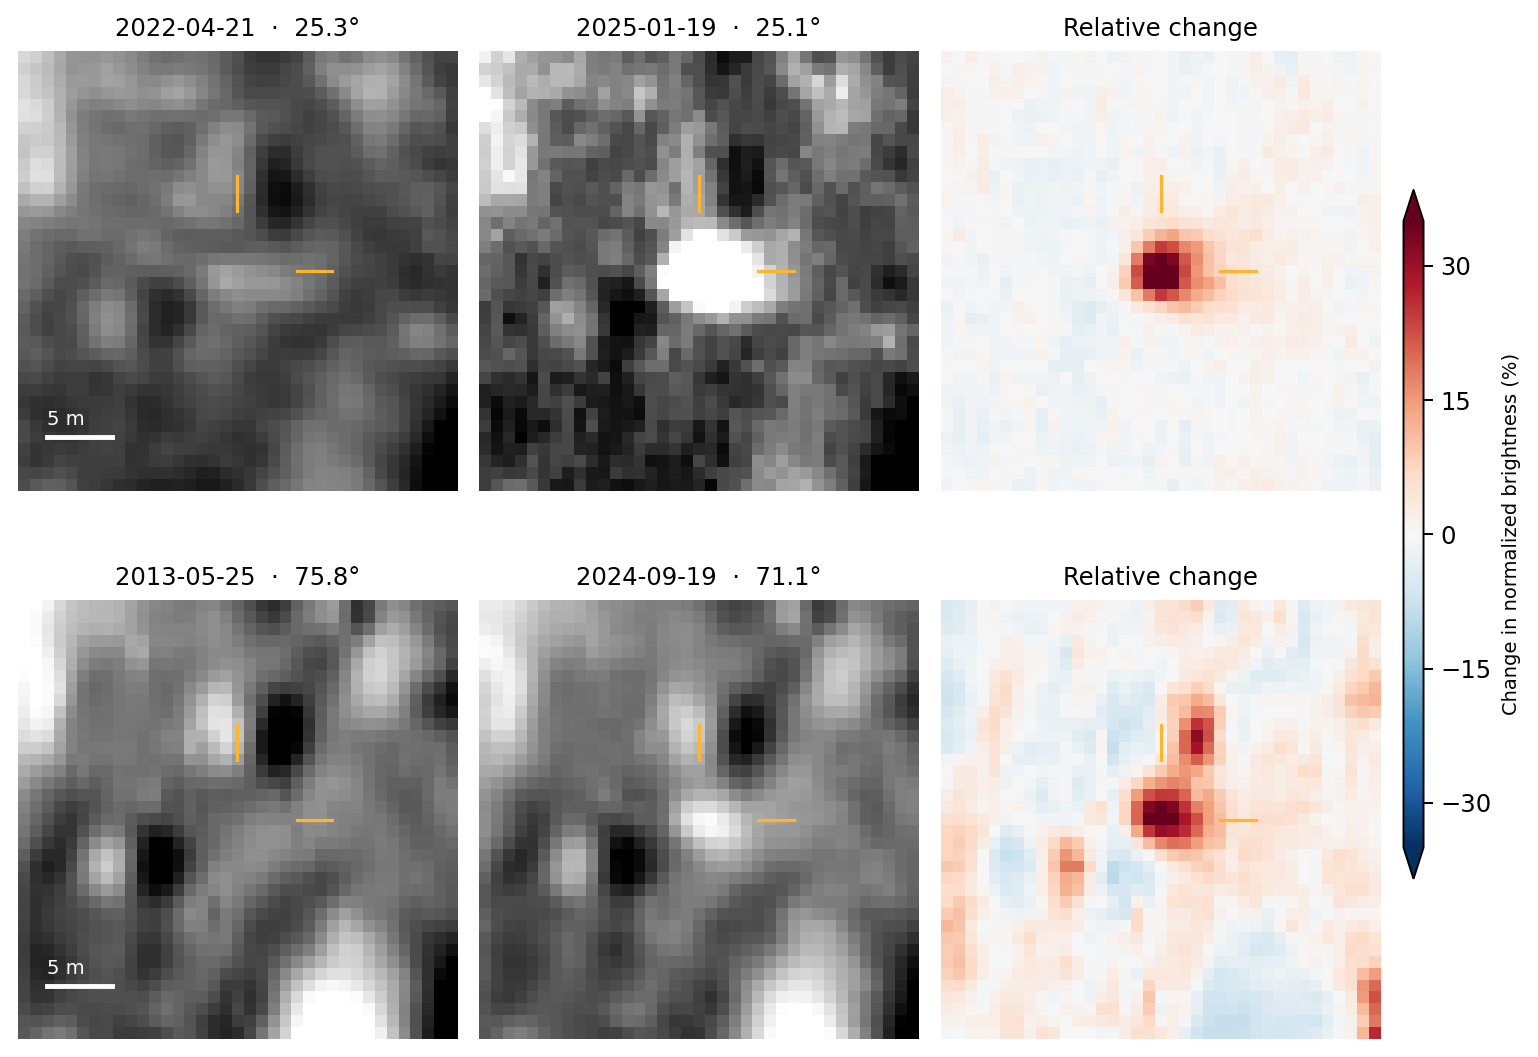
\includegraphics[width=.89\linewidth]{neliota/brightening.png}\end{center}
\figcap{\textbf{Figure 2.} PDS image pairs with similar lighting within each row. The local brightness increase in the marked central aperture is 29.8\% in the upper pair and 25.8\% in the lower pair. In the upper pair, 28 neighboring control apertures vary from $-1.5$\% to $+2.3$\%. No new rim is resolved under opposite illumination. The figures describe relative brightness and cannot establish impact origin.}

\subhead{Field coverage}
The two principal NELIOTA image pairs contain 81.57 km$^2$ (flash 281) and 117.80 km$^2$ (flash 283) of usable registered surface. A second 283 pair adds a further comparison covering 51.01 km$^2$, partially overlapping the first. A 95.40 km$^2$ farside survey found a different persistent bright mark near 7.66$^\circ$ S, 226.05$^\circ$ E, with no resolved cavity. Its relation to the approximately located N13 entry is open. In Mare Imbrium, a search for new wall-and-shadow pairs on 8.99 km$^2$ at 0.78/0.76 m per pixel produced 591 flags. Comparison with the earlier images eliminated all 591 as new resolved cavities.

The supplied archive includes native image identifiers, usable-pixel masks or coverage tables, cutouts, numerical checks, and analysis code. The field searches have no measured completeness limit for smaller or weaker features. \href{https://doi.org/10.1051/0004-6361/202449542}{Liakos et al.\ (2024)}.
\end{document}
